\documentclass[12pt]{article}
\usepackage{times} 			% use Times New Roman font

\usepackage[margin=1in]{geometry}   % sets 1 inch margins on all sides
\usepackage{hyperref}               % for URL formatting
\usepackage[pdftex]{graphicx}       % So includegraphics will work
\setlength{\parskip}{1em}           % skip 1em between paragraphs
\usepackage{indentfirst}            % indent the first line of each paragraph
\usepackage{datetime}
\usepackage[small, bf]{caption}
\usepackage{listings}               % for code listings
\usepackage{xcolor}                 % for styling code
\usepackage{multirow}

%New colors defined below
\definecolor{backcolour}{RGB}{246, 246, 246}   % 0xF6, 0xF6, 0xF6
\definecolor{codegreen}{RGB}{16, 124, 2}       % 0x10, 0x7C, 0x02
\definecolor{codepurple}{RGB}{170, 0, 217}     % 0xAA, 0x00, 0xD9
\definecolor{codered}{RGB}{154, 0, 18}         % 0x9A, 0x00, 0x12

%Code listing style named "gcolabstyle" - matches Google Colab
\lstdefinestyle{gcolabstyle}{
  basicstyle=\ttfamily\small,
  backgroundcolor=\color{backcolour},   
  commentstyle=\itshape\color{codegreen},
  keywordstyle=\color{codepurple},
  stringstyle=\color{codered},
  numberstyle=\ttfamily\footnotesize\color{darkgray}, 
  breakatwhitespace=false,         
  breaklines=true,                 
  captionpos=b,                    
  keepspaces=true,                 
  numbers=left,                    
  numbersep=5pt,                  
  showspaces=false,                
  showstringspaces=false,
  showtabs=false,                  
  tabsize=2
}

\lstset{style=gcolabstyle}      %set gcolabstyle code listing

% to make long URIs break nicely
\makeatletter
\g@addto@macro{\UrlBreaks}{\UrlOrds}
\makeatother

% for fancy page headings
\usepackage{fancyhdr}
\setlength{\headheight}{13.6pt} % to remove fancyhdr warning
\pagestyle{fancy}
\fancyhf{}
\rhead{\small \thepage}
\lhead{\small HW5, Bartels}  % EDIT THIS, REPLACE # with HW number
\chead{\small CS 432, Fall 2020} 

%-------------------------------------------------------------------------
\begin{document}

\begin{centering}
{\large\textbf{HW5 - Graph Partitioning}}\\ % EDIT THIS
                                % REPLACE # with HW num and ADD title
Logan Bartels\\                     % EDIT THIS
November 8, 2020\\                      % EDIT THIS
\end{centering}

%-------------------------------------------------------------------------


\textbf{Note: This assignment was completed in Google Collab.  All code shown in this report is copy-pasted from the notebook used to complete this assignment.  All relevant code is under the section ``HW5.''}  Here is the link to the notebook: \url{https://colab.research.google.com/drive/1IyTntJkuAC_1TGNQC7cEzKzxOPk4_v4o?usp=sharing}

\section*{Step 1}

\subsection*{Answer}

\begin{figure}[h]
    \centering
    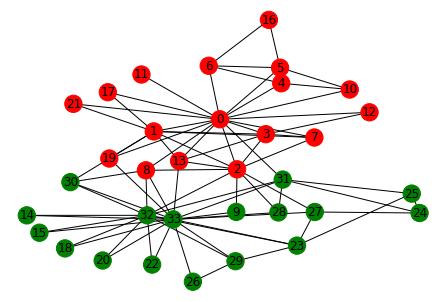
\includegraphics{step1.png}
    \caption{Force-directed original Karate Club graph.}
    \label{fig:step1Graph}
\end{figure}

\begin{lstlisting} [language=Python, caption=Python code used to complete Step 1., label=lst:step1Code]
import matplotlib.pyplot as plt
import networkx as nx

G = nx.karate_club_graph()
#G.nodes[33]["club"]

# Step 1
# Make all nodes the same color
color = ["#1f78b4"] * 34
# Loop to color nodes according to their faction
for node in G.nodes:  
  # If node belongs to Mr. Hi, color red
  if G.nodes[node]["club"] == 'Mr. Hi':
    color[node] = 'red'
  # Node belongs to John A. color green
  else:
    color[node] = 'green'
nx.draw_kamada_kawai(G, with_labels=True, node_color=color)
# plt.show()

\end{lstlisting}

\subsection*{Discussion}

The first thing in the code to note is line 5.  Originally, that line printed out the faction that the node belonged to.  I tested it on node 0 (Mr. Hi) and node 33 (John A.).  The results were ``Mr. Hi'' and ``Officer,'' respectively.  On line 9, I made every node in the graph the same color blue.  This was a precaution to catch any nodes that would not be colored by my coloring method.  Luckily, all nodes were colored.  The ``for'' loop starting on line 11 checks what ``club'' or faction the node belongs to.  If the node belongs to Mr. Hi, then it is colored red.  If the node does not belong to Mr. Hi, then it belongs to John A. or, in this case, Officer.  The node is then colored green.  The graph is force-directed, and the two factions are easily distinguishable.  The graph for this step is displayed in figure \ref{fig:step1Graph}.

\pagebreak

\section*{Step 2}

\subsection*{Algorithm}

\begin{lstlisting}[language=Python, caption=Algorithm used to remove edges from the graph., label=lst:algorithm]
# Full algorithm
# Calculate edge betweenness of all edges
edges = nx.edge_betweenness_centrality(G)
# Sort the returned dictionary by its values in descending order
sortedEdges = sorted(edges, key=edges.__getitem__, reverse=True)
# Remove the edge with the highest betweenness
G.remove_edge(sortedEdges[0][0], sortedEdges[0][1])
# Add the removed edge to a list
removedEdges.append(sortedEdges[0])
nx.draw_kamada_kawai(G, with_labels=True, node_color=color)
# plt.show()
# Check if the graph is connected
print(nx.is_connected(G))
# Show the number of connected components
print(nx.number_connected_components(G))

\end{lstlisting}

\pagebreak

\subsection*{Graphs}
\begin{figure}[h]
    \centering
    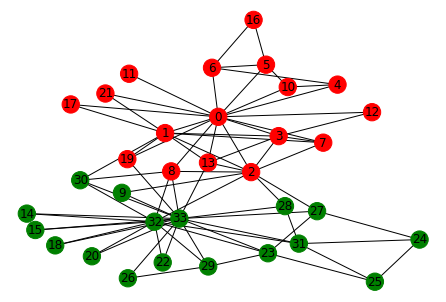
\includegraphics{iteration1.png}
    \caption{The graph after the first iteration of my Girvan-Newman-like algorithm.}
    \label{fig:iteration1}
\end{figure}

\pagebreak

\begin{figure}[h]
    \centering
    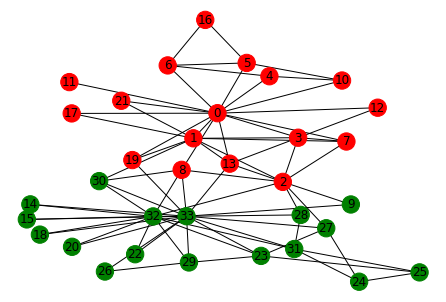
\includegraphics{iteration2.png}
    \caption{The graph after the second iteration of my Girvan-Newman-like algorithm.}
    \label{fig:iteration2}
\end{figure}

\pagebreak

\begin{figure}[h]
    \centering
    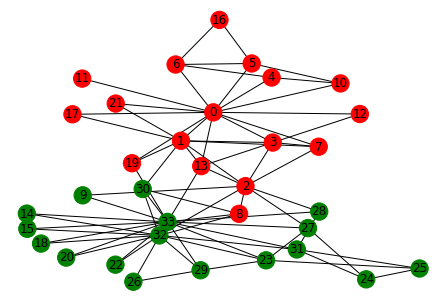
\includegraphics{iteration3.png}
    \caption{The graph after the third iteration of my Girvan-Newman-like algorithm.}
    \label{fig:iteration3}
\end{figure}

\pagebreak

\begin{figure}[h]
    \centering
    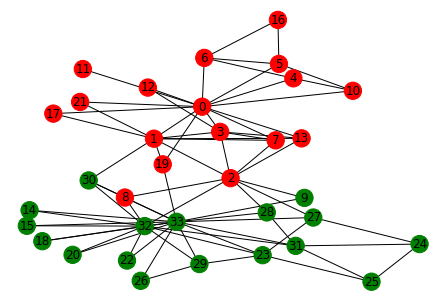
\includegraphics{iteration4.png}
    \caption{The graph after the fourth iteration of my Girvan-Newman-like algorithm.}
    \label{fig:iteration4}
\end{figure}

\pagebreak

\begin{figure}[h]
    \centering
    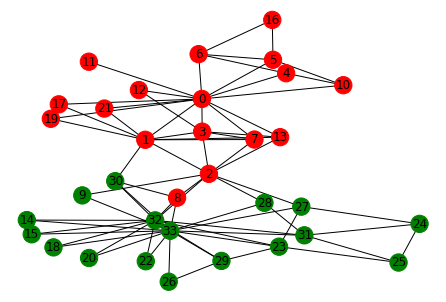
\includegraphics{iteration5.png}
    \caption{The graph after the fifth iteration of my Girvan-Newman-like algorithm.}
    \label{fig:iteration5}
\end{figure}

\pagebreak

\begin{figure}[h]
    \centering
    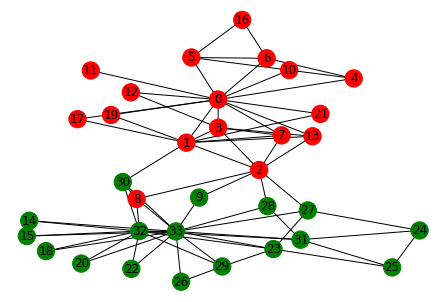
\includegraphics{iteration6.png}
    \caption{The graph after the sixth iteration of my Girvan-Newman-like algorithm.}
    \label{fig:iteration6}
\end{figure}

\pagebreak

\begin{figure}[h]
    \centering
    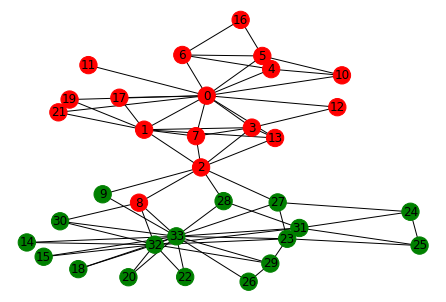
\includegraphics{iteration7.png}
    \caption{The graph after the seventh iteration of my Girvan-Newman-like algorithm.}
    \label{fig:iteration7}
\end{figure}

\pagebreak

\begin{figure}[h]
    \centering
    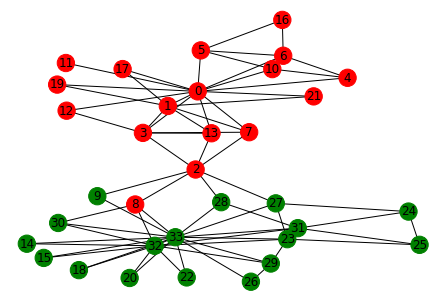
\includegraphics{iteration8.png}
    \caption{The graph after the eighth iteration of my Girvan-Newman-like algorithm.}
    \label{fig:iteration8}
\end{figure}

\pagebreak

\begin{figure}[h]
    \centering
    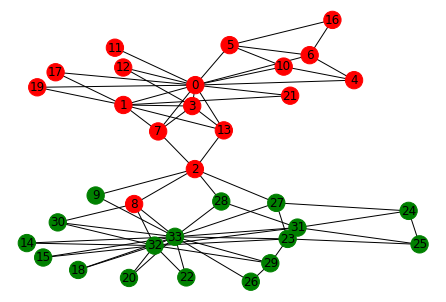
\includegraphics{iteration9.png}
    \caption{The graph after the ninth iteration of my Girvan-Newman-like algorithm.}
    \label{fig:iteration9}
\end{figure}

\pagebreak

\begin{figure}[h]
    \centering
    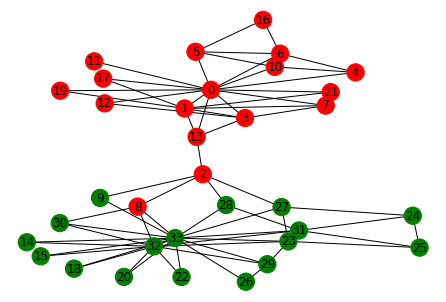
\includegraphics{iteration10.png}
    \caption{The graph after the tenth iteration of my Girvan-Newman-like algorithm.}
    \label{fig:iteration10}
\end{figure}

\pagebreak

\begin{figure}[h]
    \centering
    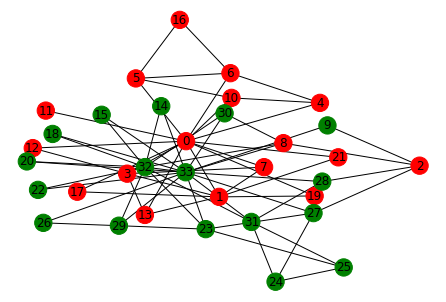
\includegraphics{iteration11.png}
    \caption{The graph after the eleventh iteration of my Girvan-Newman-like algorithm.}
    \label{fig:iteration11}
\end{figure}

Because the graph got rather messy after the eleventh iteration, I inserted a circular version of the step1 graph and a circular version of the iteration11 graph on the next two pages.  The circular step1 graph is for comparison to the circular version of the iteration11 graph.  I did attempt to run more iterations in the hope of the graph looking neater to no avail, hence the circular graphs.

\pagebreak

\begin{figure}[h]
    \centering
    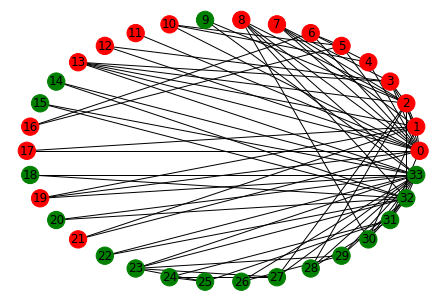
\includegraphics{circularStep1.png}
    \caption{A circular version of the original Karate Club graph used in step1 for comparison to the circular version of iteration11.}
    \label{fig:circStep1}
\end{figure}

\pagebreak

\begin{figure}[h]
    \centering
    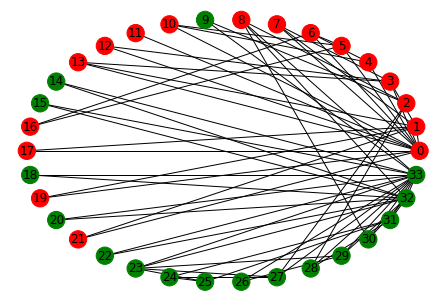
\includegraphics{circularIteration11.png}
    \caption{A circular version of the graph after the eleventh iteration.}
    \label{fig:circIteration11}
\end{figure}

\pagebreak

\subsection*{Discussion}
Starting with my edge-removal algorithm in listing \ref{lst:algorithm}, the edge betweenness of every edge is calculated by the ``edge\_betweenness\_centrality'' function on line 3.  The dictionary returned by the function is stored in the ``edges'' variable.  The dictionary stored in the ``edges'' variable was copy-pasted into ``edges.txt.''  The file contents are displayed in listing \ref{lst:edges}.  \textbf{Please note that the dictionary displayed consists of the betweenness of every edge of the original graph;} no edges have been removed.  It is only meant to illustrate the data container.  On line 5, the keys (edges) in the ``edges'' dictionary are sorted by their values (betweenness) in descending order, and stored in the ``sortedEdges'' variable.  The resulting list of tuples stored in the ``sortedEdges'' variable was copy-pasted into ``sortedEdges.txt.''  The file contents are displayed in listing \ref{lst:sortedEdges}.  Like ``edges.txt,'' no edges have been removed.  On line 7, the first edge in ``sortedEdges'' (the edge with the highest betweenness) is removed.  Something to note: since this was done in Google Collab, lines 3 and 5 are redone every time the code is executed.  So after an edge is removed, the betweenness values are recalculated and re-sorted.  This assures that the edge with the highest betweenness is removed every iteration.  When an edge is removed, it is appended to a list called ``removedEdges.''  Note that in the Collab notebook,  ``removedEdges'' was declared as an empty list in the cell above the algorithm, and it is not shown in the report.  The content of ``removedEdges'' was copy-pasted into ``removedEdges.txt.''  The contents of ``removedEdges.txt'' are displayed in listing \ref{lst:remEdges}.  The graph is then drawn.  Then the value (true or false) of the ``is\_connected'' function is printed, along with the number of connected components of the graph using the ``number\_connected\_components'' function.

The algorithm was executed manually until the ``is\_connected'' function returned ``false.''  This took eleven iterations.  Once the graph was no longer one connected component, the ``number\_connected\_components'' function printed out ``2.''  This meant the graph consisted of two connected components.  Because it was difficult to see the disconnected components of the graph in figure \ref{fig:iteration11}, I plotted a circular version in figure \ref{fig:circIteration11}.  I also took the liberty of providing a circular version of the graph in figure \ref{fig:step1Graph} for comparison.  It is shown in figure \ref{fig:circStep1}.

\lstinputlisting[caption=Dictionary with edges as keys and their betweenness as values, label=lst:edges]{edges.txt}

\lstinputlisting[caption=List of tuples that consists of edges sorted by their betweenness in descending order., label=lst:sortedEdges]{sortedEdges.txt}

\lstinputlisting[caption=List of tupes that contains the removed edges of the Karate Club graph., label=lst:remEdges]{removedEdges.txt}

\section*{Step 3}
\textbf{Note: I will be comparing figures \ref{fig:circStep1} and \ref{fig:circIteration11}}.

The first difference to note is the step1 graph has only one connected component.  The graph after eleven iterations has two connected components.  Something I noticed between the two graphs is after eleven iterations, there were edges removed between red nodes, red and green nodes, but not green nodes.  Comparing the list of removed edges to the nodes in the graph corroborates this.  I counted six edges between red nodes removed, and five edges between red and green nodes removed.  Given the amount of edges removed between nodes belonging to Mr. Hi (red nodes), I'm not sure that this particular split could have been predicted by the weighted graph of social interactions.  I would think that like-minded people (in this case, people that belong to Mr. Hi's club; red nodes) would have a stronger connection than than those who think differently (red and green nodes).  Perhaps the takeaway here is that you never really know somebody.

\pagebreak

\section*{References}

\begin{itemize}
    \item {NetworkX edge\_betweenness\_centrality, \url{https://networkx.org/documentation/stable/reference/algorithms/generated/networkx.algorithms.centrality.edge\_betweenness\_centrality.html?highlight=edge\_betweenness\_centrality#networkx.algorithms.centrality.edge\_betweenness\_centrality}}
    \item {NetworkX karate\_club\_graph, \url{https://networkx.org/documentation/stable/reference/generated/networkx.generators.social.karate\_club\_graph.html?highlight=karate\_club\_graph#networkx.generators.social.karate\_club\_graph}}
    \item {Python Dictionaries, \url{https://www.w3schools.com/python/python_dictionaries.asp}}
    \item {How to Sort Python Dictionaries by Key or Value, \url{https://www.pythoncentral.io/how-to-sort-python-dictionaries-by-key-or-value/#:~:text=Sorting\%20Python\%20dictionaries\%20by\%20Keys.\%20If\%20we\%20want,has\%20been\%20sorted\%20\%28in\%20ascending\%20order\%20by\%20default\%29.}}
    \item {NetworkX remove\_edge, \url{https://networkx.org/documentation/stable/reference/classes/generated/networkx.Graph.remove\_edge.html?highlight=remove\_edge#networkx.Graph.remove\_edge}}
    \item {NetworkX is\_connected, \url{https://networkx.org/documentation/stable/reference/algorithms/generated/networkx.algorithms.components.is\_connected.html?highlight=is\_connected#networkx.algorithms.components.is\_connected}}
    \item {NetowrkX number\_connected\_components, \url{https://networkx.org/documentation/stable/reference/algorithms/generated/networkx.algorithms.components.number\_connected\_components.html?highlight=number\_connected\_components#networkx.algorithms.components.number\_connected\_components}}
    \item {Week-07 Slides, \url{https://docs.google.com/presentation/d/1FzrzxRzslE20nWOjb_uM8jz2xvT1IOOZ9uIoYVjco7s/edit#slide=id.g30f264e945_1_6}}
    \item {Week-09 Slides, \url{https://docs.google.com/presentation/d/1POtPTmBw6MSBI7qIT85uT8DPndWcQzGpEaZQtySr1R0/edit#slide=id.g311d60d551_0_6}}
    \item {An Information Flow Model for Conflict and Fission in Small Groups, \url{http://aris.ss.uci.edu/~lin/76.pdf}}
\end{itemize}

\end{document}

